\section{Networks in molecular biology}

% Make the case for pathways and gene interactions - Why it is important to study them
Interactions and the relationships between multiple components are central to tissues functioning and biological processes. There are multiple levels of interactions in the molecular biology which are represented by gene pathways, where one gene influences another to produce more or less of a protein, and that in turn produces more proteins and so on until that pathway fulfil its function. When something goes wrong in the body as in the case of the cancer, a certain pathways is altered and it is not working as intended. Thus, it is understandable why the field of using networks to analyse genomic data is saw rapid and exciting advancements in the recent years. 
 
% Introduce graph and network theory
Network or graph theory is the branch of the mathematics that models the interactions between multiple elements. \Cref{fig:lit:basic_net} shows a simple graph where the nodes/vertices represent the genes and the edges/links the connection's strength between.

% Need to address the network pathways 
There has been a lot of work on analysing the pathways which is covered in \cref{s:lit:multi-view}. However, the information about pathways is generally incomplete, in continuous research and a complete representation of a tissue is simply not available for most of the tissues. Therefore, there are other alternatives to analyse the gene interactions in a tissue.

\begin{figure}[!htb]
  \centering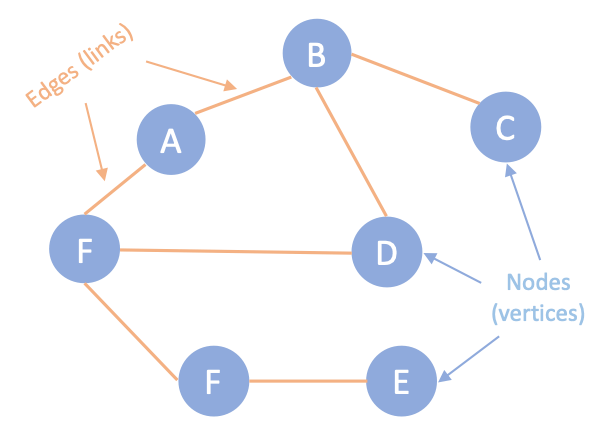
\includegraphics[width=0.5\textwidth,height=0.5\textheight,keepaspectratio]{Sections/Lit_review/Resources/basic_graphs.png}
    \caption{Basic graphs.}
    \label{fig:lit:basic_net}
\end{figure}
\FloatBarrier



% Why are we choosing the co-expressed networks?
One such approach are the co-expressed networks which uses different correlation metrics (e.g. Spearman, Pearson or partial-correlation) from gene expression to model the strengths between the nodes (edges). The rationale behind is that genes expressed together have a higher correlation will also have a stronger connection between nodes,conversely, genes with a weaker connection are represented are lower correlated. After the network is built related genes are grouped together in communities which are then used to subtype the disease. This approaches are covered in Section \ref{s:lit:co_net} and it is the method used in this project as it offers a more convenient and adaptable method to other diseases or other data (multiple sources of gene expression).

% DEA as an alternative
Another alternative to co-expressed network is to build the network based on the Deferentially Expressed Analysis (DEA) data between the healthy and tumour. While being a more restrictive approach this approach will highlight the differences between the two tissue states and might provide new biological insights. The review \citet{Van_Dam2018-id} covers such network approaches and also acts as guide on building DEA-based networks. Using DEA between healthy and tumours was considered in the project but the co-expressed network was preferred for its versatility.

% Alternative methods for co-expressed networks - in the review from Petti
The review from 2023 of \citet{Petti2023-qo} is covering the different network methods used in the field to stratify a disease a few which are explored in this project. The patient similarity network section covers different methods using co-expression networks but not the work of \citet{Care2019-ij} on PGCNA (2019) which is one of the main sources of inspiration in this project. Nevertheless, the review offers good insights on the other alternatives such as the network-based stratification (NBS), initially proposed for integrating data by \citet{Hofree2013-ld} and it is covered in \cref{s:lit:net_prop}, or the multi-layer (\cref{s:lit:multi-layer}) networks.

This chapter covers the work on co-expressed networks with a focus on PGCNA and WGCNA, as well as some research done using partial-correlation as an alternative to the standard methods (Spearman, Pearson) to build a graph. As an alternative to this approach the networks constructed using a Bayesian approach is covered in the next section. \Cref{s:lit:net_data_int} covers network propagation and multi-layer graphs as methods to integrate multiple data types. Lastly, the \cref{s:lit:comm_detect} is dedicated to community detection algorithms as they have a very important role in finding the groups of genes with a biological function.

\import{Sections/Lit_review/}{co-expressed_net.tex}

\import{Sections/Lit_review/}{comm_detection.tex}


% Remarks
\subsection{Conclusion} 

This section explored some of the popular methods to build network and how these models were applied to a variety of diseases. The co-expressed networks, with WGCNA \cite{Langfelder2008-sn} being the most popular method and PGCNA \cite{Care2019-ij} introducing a newer correlation based networks. HCNM \cite{Vangimalla2021-fc} and iHNMMO \citet{Peng2017-ik} create multi-layer networks each being a representation of the data types. While DrDimont \cite{Hiort2022-lk} and NetICS \citet{Dimitrakopoulos2018-br} uses differentially expressed analysis results between either healthy-disease or disease-drug response to build the networks. Partial-correlation has also been in network construction phase by \citet{De_la_Fuente2004-ts} as well as Bayesian approaches  probabilistic methods by \cite{Nakazawa2021-yq, Tamada2011-ok, Tanaka2020-mw}.

All of these methods shared their aim to advance the understanding and analysis of the genomic data, but differ in their objectives. Only PGCNA, WGCNA, HCNM and Nakazawa et al.\cite{Care2019-ij, Langfelder2008-sn, Nakazawa2021-yq,  Vangimalla2021-fc} were developed to subtype the cancer. iHNMMO \cite{Peng2017-ik}, NetICS \cite{Dimitrakopoulos2018-br} have the goals to find a subset of relevant genes at the disease level, while DrDimont \cite{Hiort2022-lk} the genes responding to a drug. 

% Argument for why chossing correlation - not great
In this project, the approach taken is similar to the one from PGCNA and WGCNA which is to built the network from correlation scores of the data. Despite the casual-inference limitations, the correlation based networks are computational faster, simpler to implement and easier to analyse, which is a fundamental aspect of the project.





% PGCNA 

% The other paper with DEA
